\chapter{Resultats}
\label{c:Resultats}

Un cop finalitzada la recerca, passem a la part pràctica. Tal com vam indicar als objectius, el nostre principal propòsit era construir una xarxa neuronal de tipus regressió, que analitza les dades disponibles i genera una predicció numèrica contínua. En aquest capítol mostrarem els resultats que hem aconseguit en aquest TR.


\section{Xarxa neuronal de regressió}\label{sec:op}

Una xarxa neuronal de regressió, a diferència d’altres tipus de xarxes, té una sortida lineal que permet predir un valor numèric continu. Aquestes xarxes necessiten un conjunt de dades ampli i ben estructurat perquè puguin aprendre les relacions entre les variables d’entrada i generar prediccions fiables.\\[0.2cm]
A continuació es mostra un esquema representatiu d’una xarxa neuronal de regressió:

\begin{figure}[h!]
\centering
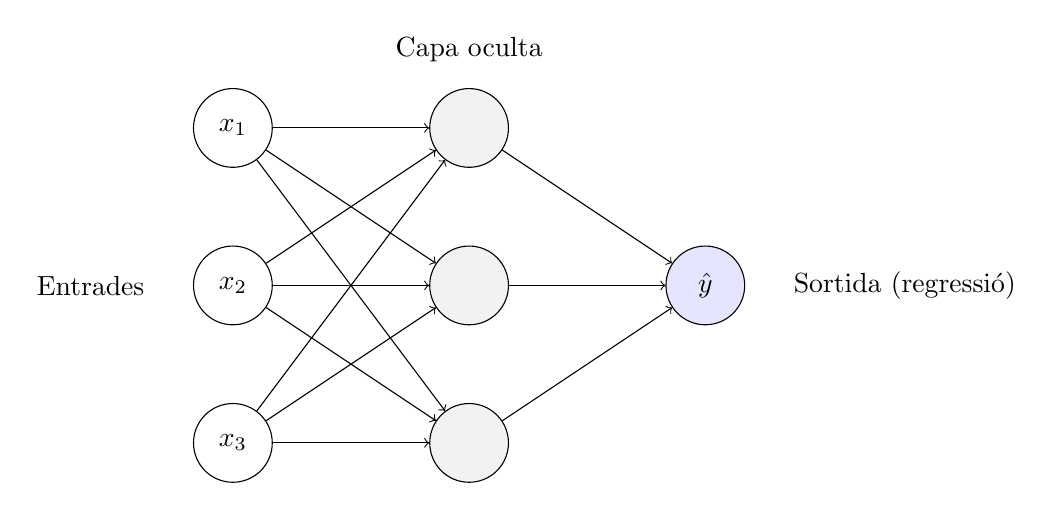
\begin{tikzpicture}[scale=1, transform shape]


\node[circle, draw, minimum size=1cm] (I1) at (0,2) {$x_1$};
\node[circle, draw, minimum size=1cm] (I2) at (0,0) {$x_2$};
\node[circle, draw, minimum size=1cm] (I3) at (0,-2) {$x_3$};


\node[circle, draw, fill=gray!10, minimum size=1cm] (H1) at (3,2) {};
\node[circle, draw, fill=gray!10, minimum size=1cm] (H2) at (3,0) {};
\node[circle, draw, fill=gray!10, minimum size=1cm] (H3) at (3,-2) {};


\node[circle, draw, fill=blue!10, minimum size=1cm] (O1) at (6,0) {$\hat{y}$};


\foreach \i in {1,2,3}
\foreach \h in {1,2,3}
\draw[->] (I\i) -- (H\h);


\foreach \h in {1,2,3}
\draw[->] (H\h) -- (O1);


\node[left] at (-1,0) {Entrades};
\node at (3,3) {Capa oculta};
\node[right] at (7,0) {Sortida (regressió)};

\end{tikzpicture}
\caption{Esquema d’una xarxa neuronal de regressió}
\end{figure}

Abans de crear la xarxa neuronal, vam definir quin seria el seu objectiu: predir les notes finals de matemàtiques dels alumnes. Les dades es van recollir mitjançant un formulari que incloïa les següents preguntes:

\begin{enumerate}
    \item Realització de deures
    \item Hores d’estudi setmanals
    \item Hores de son
    \item Interès en la matèria
    \item Nota del segon trimestre
    \item Nota del tercer trimestre
    \item Nota final
\end{enumerate}

D’aquesta manera, la xarxa neuronal aprendrà a predir les notes dels alumnes comprenent la relació entre les dades d’entrada i el resultat final.\\[0.2cm]
Per recollir les respostes vam utilitzar Google Drive per crear el formulari i el vam compartir en diversos grups de WhatsApp de batxillerat. Finalment, vam obtenir 18 respostes, tal com es mostra a la imatge següent:

\begin{figure}[h!]
\centering
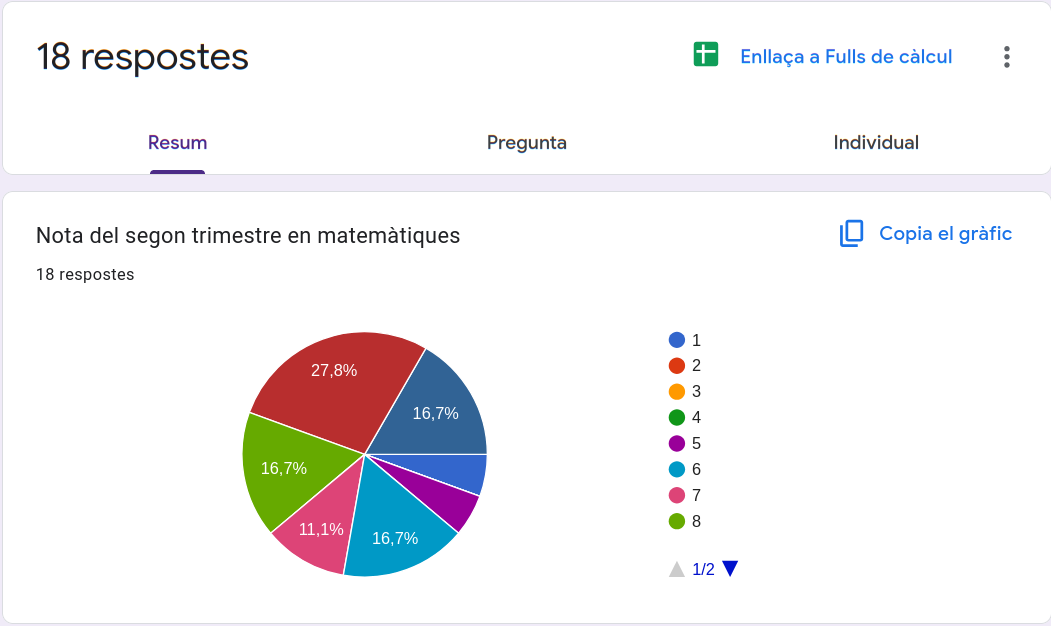
\includegraphics[width=1\textwidth]{./figures/Formulari.png}
\caption{Resposta a una de les preguntes del formulari}
\end{figure}

Un cop recopilades les dades necessàries, vam iniciar la construcció de la xarxa neuronal.

\section{Xarxa Neuronal amb llenguatge de programació}\label{sec:10}
En aquest apartat explicarem pas a pas la creació de la nostra xarxa neuronal de regressió amb un llenguatge de programació.

\subsection{De Celcius a Fahrenheit}

Abans de començar a treballar amb la xarxa neuronal definitiva, vam crear-ne una de més simple per comprendre millor el funcionament d’una xarxa neuronal de regressió. En aquest cas, vam triar un convertidor d’unitats de temperatura, de Celsius (unitat basada en el punt de fusió de l’aigua) a Fahrenheit (sistema basat en els punts d’ebullició i congelació de l’aigua). Aquesta xarxa la vam desenvolupar amb el llenguatge de programació Python. Una explicació detallada es pot trobar a l’apèndix~\ref{a:CelsiusFahrenheit}:~\nameref{a:CelsiusFahrenheit}.


\subsection{Predicció de les notes finals de matemàtiques}
Un cop desenvolupada la xarxa neuronal de Celsius a Fahrenheit, vam poder començar a crear la xarxa neuronal principal que ens havíem proposat. Per iniciar el procés, vam importar els frameworks i les biblioteques necessàries: \texttt{numpy}, \texttt{TensorFlow}, \texttt{matplotlib}, \texttt{MinMaxScaler}, \texttt{random} i \texttt{os}.

\begin{itemize}

\item \textbf{MinMaxScaler: } eina de la llibreria \texttt{sklearn} que normalitza les dades, convertint-les dins del rang $[0,1]$ i facilitant que la xarxa neuronal interpreti correctament les relacions numèriques.

\item \textbf{random: } llibreria bàsica de Python que permet generar i seleccionar nombres aleatoris.

\item \textbf{os: } llibreria estàndard de Python que facilita la interacció amb el sistema operatiu.

\end{itemize}

\begin{figure}[h!]
\centering
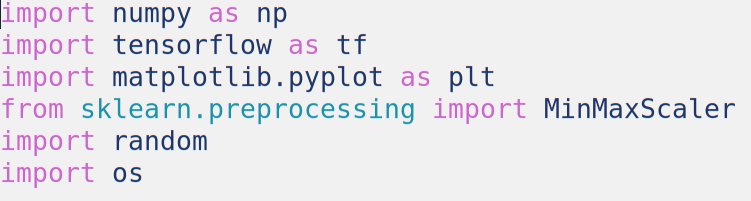
\includegraphics[width=0.5\textwidth]{./figures/21.png}
\caption{Biblioteques i frameworks utilitzats}
\end{figure}

A diferència de la xarxa anterior, vam fixar els resultats de la predicció per garantir que les notes finals siguin reproduïbles. Tot i que amb \texttt{random} es podria seleccionar qualsevol nombre, vam assignar la llavor (\texttt{seed}) amb el valor 42. D’aquesta manera, la xarxa sempre s’inicialitzarà amb els mateixos pesos i biaixos.\\[0.2cm]
També vam controlar l’aleatorietat de les diferents llibreries, com \texttt{NumPy}, \texttt{TensorFlow} i \texttt{random}, i vam establir el valor del hash de Python amb \texttt{os}.
Control de l’aleatorietat:
\begin{itemize}
\item \textbf{Llavor:} \texttt{seed = 42}
\item \textbf{NumPy:} \texttt{np.random.seed(seed)}
\item \textbf{TensorFlow:} \texttt{tf.random.set\_seed(seed)}
\item \textbf{random:} \texttt{random.seed(seed)}
\item \textbf{Python:} \texttt{os.environ["PYTHONHASHSEED"] = str(seed)}
\end{itemize}

\begin{figure}[h!]
\centering
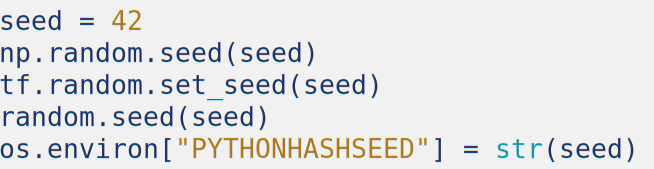
\includegraphics[width=0.5\textwidth]{./figures/22.png}
\caption{Fixació dels seeds}
\end{figure}

Un cop vam fixar els pesos i biaixos, vam emmagatzemar les dades per a l’entrenament. Les dades d’entrada es representen amb \texttt{X}, seguint l’ordre de variables següent:

\begin{enumerate}
\item Realització de deures
\item Hores d’estudi setmanals
\item Hores de son
\item Interès en la matèria
\item Nota del segon trimestre
\item Nota del tercer trimestre
\end{enumerate}

Definim \texttt{X = np.array([])}, creant així una llista que anirem omplint amb les dades del formulari. L’estructura ha de ser sempre \texttt{[x1, x2, x3, x4, x5, x6]} amb \texttt{dtype=float}, ja que treballem amb nombres decimals.

La sortida, \texttt{y}, tindrà una sola fila amb els valors de les notes recollides al formulari.

\begin{figure}[h!]
\centering
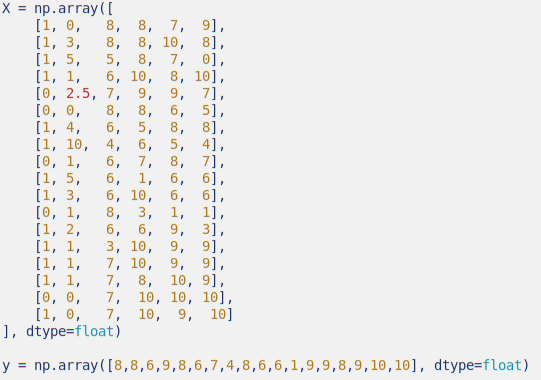
\includegraphics[width=0.7\textwidth]{./figures/23.png}
\caption{Emmagatzematge de les dades}
\end{figure}

La normalització és crucial perquè la xarxa entengui millor les relacions entre les dades, ja que els valors poden variar molt (hores d’estudi, notes i altres mesures). Per això utilitzem \texttt{MinMaxScaler} tant per \texttt{X} com per \texttt{y}.

\begin{itemize}
\item Creem l’escalador amb \texttt{scaler = MinMaxScaler()}
\item Normalitzem \texttt{X} amb \texttt{X\_scaled = scaler.fit\_transform(X)}
\item Normalitzem \texttt{y} amb \texttt{scaler\_y} i \texttt{y\_scaled = scaler\_y.fit\_transform(y.reshape(-1,1))}
\end{itemize}

\begin{figure}[H]
\centering
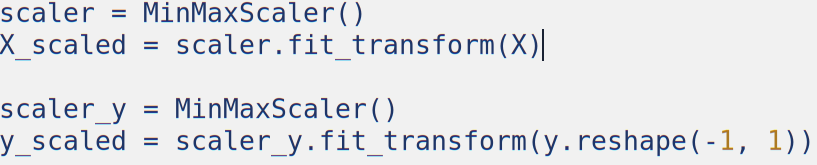
\includegraphics[width=0.5\textwidth]{./figures/24.png}
\caption{Normalització de les dades}
\end{figure}

\begin{figure}[H]
\centering
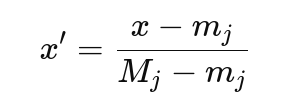
\includegraphics[width=0.3\textwidth]{./figures/25.png}
\caption{Normalització Min-Max\cite{Min-Max}}
\end{figure}

A continuació, definim l’estructura de la xarxa neuronal amb un model seqüencial:
\begin{itemize}
\item \textbf{Primera capa oculta:}\
\texttt{tf.keras.layers.Dense(32, activation="relu", input\_shape=[6])}
Definim 32 neurones amb funció d’activació ReLU. L’entrada té 6 característiques corresponents a \texttt{X}.

\item \textbf{Segona capa oculta:}\
\texttt{tf.keras.layers.Dense(16, activation="relu")}
Conté 16 neurones amb activació ReLU. L’entrada es dedueix automàticament de la capa anterior.

\item \textbf{Capa de sortida:}\
\texttt{tf.keras.layers.Dense(1)}
Una sola neurona per obtenir la predicció de la nota final. No s’aplica cap funció d’activació per mantenir la relació lineal.
\end{itemize}

\begin{figure}[h!]
\centering
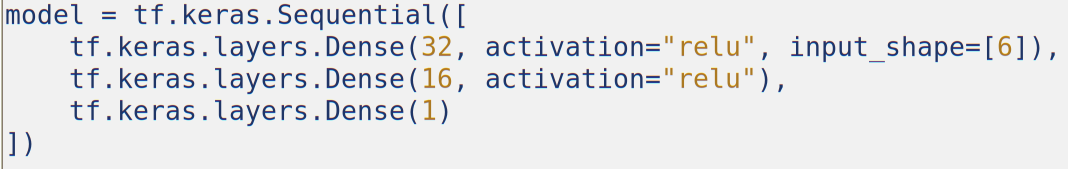
\includegraphics[width=0.7\textwidth]{./figures/26.png}
\caption{Estructura de la xarxa neuronal}
\end{figure}

Compilació del model amb \texttt{.compile()}:

\begin{itemize}
\item \textbf{Optimitzador:} \texttt{tf.keras.optimizers.Adam(0.01)}
Optimitzador adaptatiu que ajusta automàticament la taxa d’aprenentatge dels pesos durant l’entrenament.

\item \textbf{Funció de pèrdua:} \texttt{"mean\_squared\_error"}
Mesura la diferència entre els valors reals i les prediccions, penalitzant fortament els errors grans per millorar la precisió del model.

\item \textbf{Mètrica:} \texttt{["mae"]}
Calcula l’error absolut mitjà entre les prediccions i els valors reals, proporcionant una mesura intuïtiva del rendiment del model.
\end{itemize}

\begin{figure}[H]
\centering
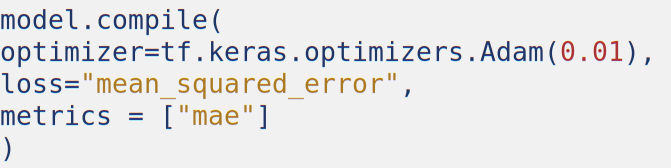
\includegraphics[width=0.5\textwidth]{./figures/27.png}
\caption{Configuració de la xarxa}
\end{figure}

L’entrenament del model es realitza amb la funció \texttt{.fit()}, utilitzant \texttt{X\_scaled} i \texttt{y\_scaled} durant 400 èpoques. S’estableix \texttt{verbose=1} per mostrar el progrés de l’entrenament i l’error corresponent a cada època.
\begin{figure}[H]
\centering
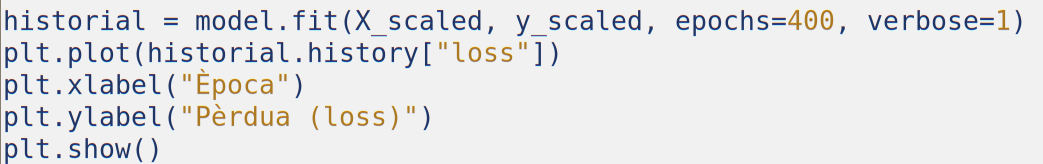
\includegraphics[width=0.7\textwidth]{./figures/28.png}
\caption{Entrenament de la xarxa i la corba de pèrdua}
\end{figure}

Per tal predir una nova mostra:
\begin{itemize}
\item Normalització de l’entrada: \texttt{nou\_entrada\_scaled = scaler.transform(nou\_entrada)}
\item Predicció amb la xarxa: \texttt{prediccio = model.predict(nou\_entrada\_scaled)}
\item Transformació inversa de la normalització: \texttt{prediccio\_real = scaler\_y.inverse\_transform(prediccio)}
\item Mostra del resultat: \texttt{print("Nota prevista:", round(prediccio\_real[0][0],2))}
\end{itemize}

\begin{figure}[h!]
\centering
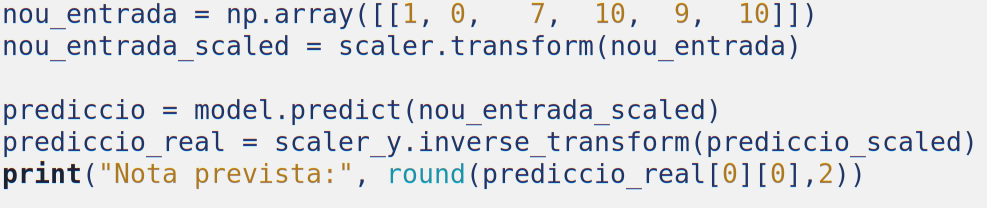
\includegraphics[width=0.7\textwidth]{./figures/29.png}
\caption{Resultat final i ajustaments}
\end{figure}

% \begin{figure}[h!]
% \centering
% 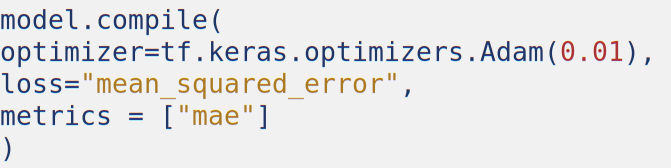
\includegraphics[width=0.5\textwidth]{./figures/27.png}
% \caption{Configuració de la xarxa}
% \end{figure}

% Entrenament del model amb \texttt{.fit()} utilitzant \texttt{X\_scaled} i \texttt{y\_scaled} durant 400 èpoques, amb \texttt{verbose=1} per mostrar el progrés i l’error per època.
%
% \begin{figure}[h!]
% \centering
% 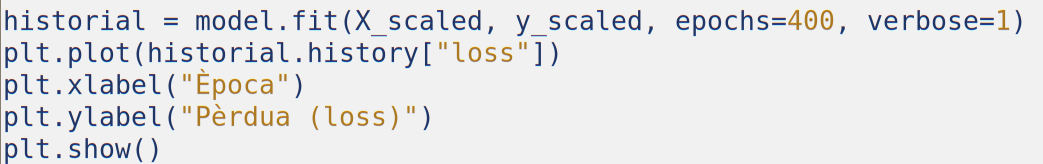
\includegraphics[width=0.7\textwidth]{./figures/28.png}
% \caption{Entrenament de la xarxa i corba de pèrdua}
% \end{figure}
%
% Per predir una nova mostra:
%
% \begin{itemize}
% \item Normalització de l’entrada: \texttt{nou\_entrada\_scaled = scaler.transform(nou\_entrada)}
% \item Predicció amb la xarxa: \texttt{prediccio = model.predict(nou\_entrada\_scaled)}
% \item Transformació inversa: \texttt{prediccio\_real = scaler\_y.inverse\_transform(prediccio)}
% \item Mostra del resultat: \texttt{print("Nota prevista:", round(prediccio\_real[0][0],2))}
% \end{itemize}
%
% \begin{figure}[H]
% \centering
% 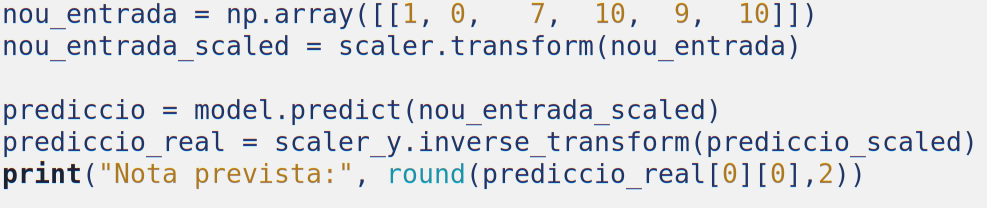
\includegraphics[width=0.5\textwidth]{./figures/29.png}
% \caption{Resultat final i ajustaments}
% \end{figure}
\clearpage
\section{Xarxa Neuronal amb full de càlcul}\label{sec:11}
En aquest apartat continuarem treballant amb la xarxa neuronal de regressió, però aquesta vegada utilitzarem un full de càlcul.
L’estructura que emprarem per a aquesta pràctica serà la del perceptró.

\begin{figure}[h!]
    \centering
    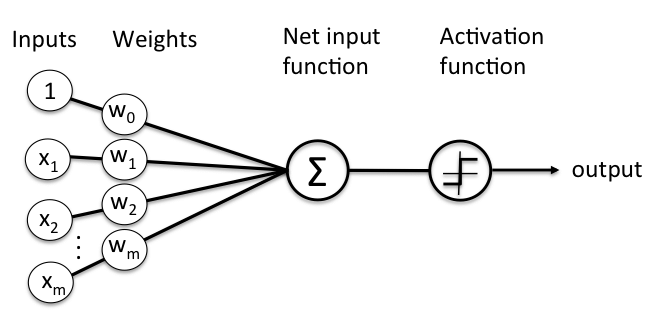
\includegraphics[width=0.6\textwidth]{./figures/perceptro.png}
    \caption{Estructura del perceptró.~\cite{Img_perceptro}}
\end{figure}

Iniciem ordenant les dades de cada alumne del formulari en el full de càlcul.
\begin{figure}[H]
    \centering
    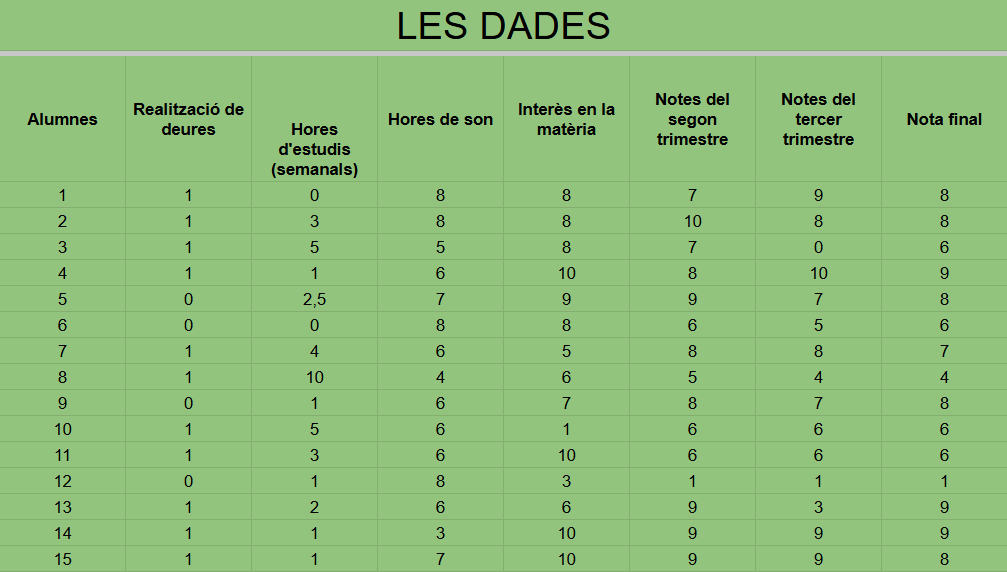
\includegraphics[width=0.8\textwidth]{./figures/Dades.png}
    \caption{Dades dels alumnes en el full de càlcul}
\end{figure}
Un cop ordenada tota la informació, decidim representar els valors d’entrada d’una manera més senzilla i compacta, anomenant-los $x_i$.
\clearpage
\begin{itemize}
 \item \textbf {Realització dels deures:} X1
 \item \textbf {Hores d'estudi:} X2
 \item \textbf {Hores de son:} X3
 \item \textbf {Interès en la matèria:} X4
 \item \textbf {Notes del segon trimestre:} X5
 \item \textbf {Notes del tercer trimestre:} X6
 \item \textbf {Nota final:} Y
\end{itemize}

Aquesta representació queda així:

\begin{figure}[h!]
    \centering
    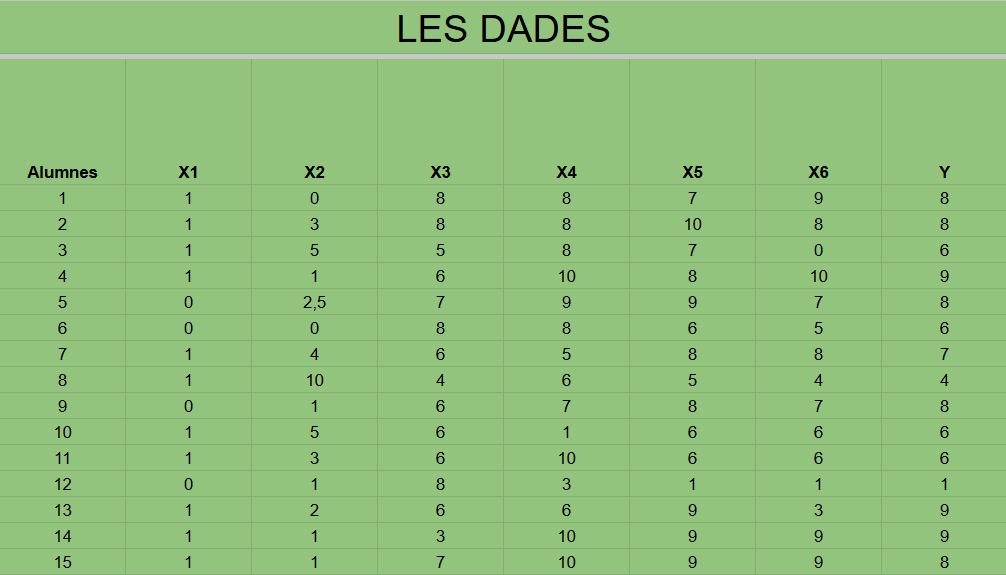
\includegraphics[width=0.9\textwidth]{./figures/Dades_resumides.png}
    \caption{Taula resumida}
\end{figure}

L'entrada ``Realització de deures'' és una dada binària que només pot prendre valors 0 o 1.
\subsection{Normalització de dades}\label{subsec:24}
Abans de continuar, recordem què és la normalització de dades.
La normalització de dades és una tècnica de processament que consisteix a transformar dades amb diferents escales a una escala comuna. Això facilita la comparació i l’anàlisi per part de la xarxa neuronal i millora el seu rendiment. \\En el nostre cas, disposem de dades binàries i dades ordinàries que poden prendre qualsevol valor; aquest desequilibri podria afectar els càlculs posteriors si no es resol.
Per aquesta raó, convertim totes les dades en valors compresos entre 0 i 1. Aquest procés implica calcular la mitjana i la desviació estàndard de cada variable. Per fer-ho, utilitzem la fórmula següent:
$$z = \frac{x - \mu}{\sigma}$$
\begin{center}
    $z$ és el valor normalitzat\\
    $x$ és el valor original\\
    $\mu$ és la mitjana\\
    $\sigma$ és la desviació típica
\end{center}


Aquests càlculs són fàcils d'obtenir amb les funcions que ens proporciona el full de càlcul.

\begin{figure}[H]
    \centering
    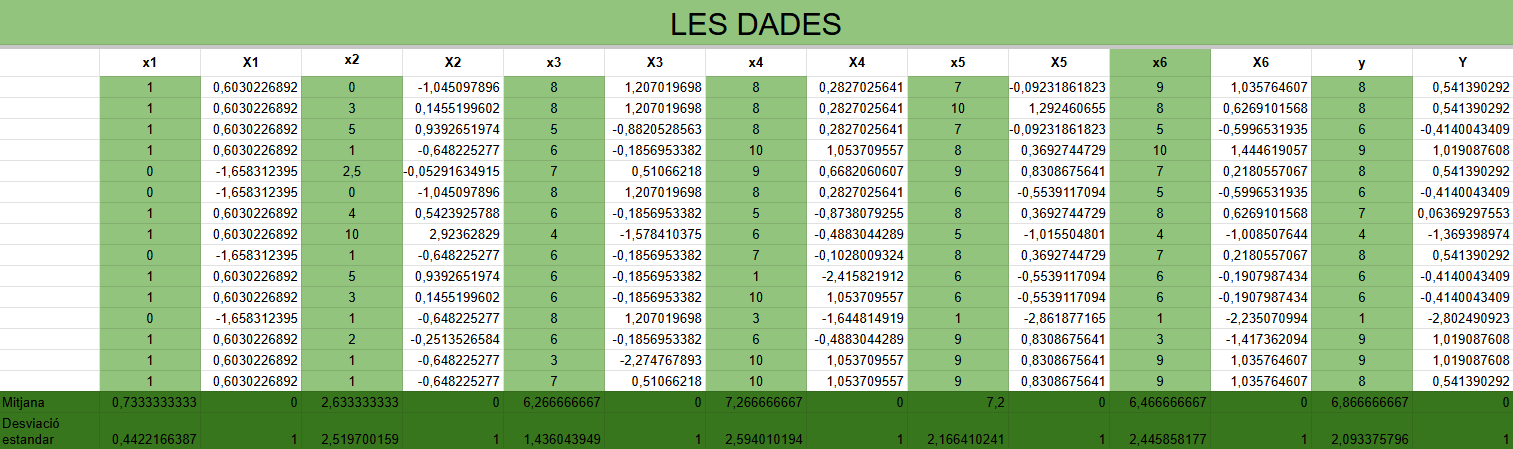
\includegraphics[width=1\textwidth]{./figures/Dades_normalitzades.png}
    \caption{Taula resumida}
\end{figure}
\subsection{Els paràmetres del model}
Ara que tenim totes les dades preparades, assignem a cada variable $X$ un pes per determinar la seva importància en la predicció final. Al començament de l’entrenament, assignem a tots els valors d’entrada el mateix pes, ja que aquests es corregiran gradualment durant el procés.

\begin{figure}[H]
    \centering
    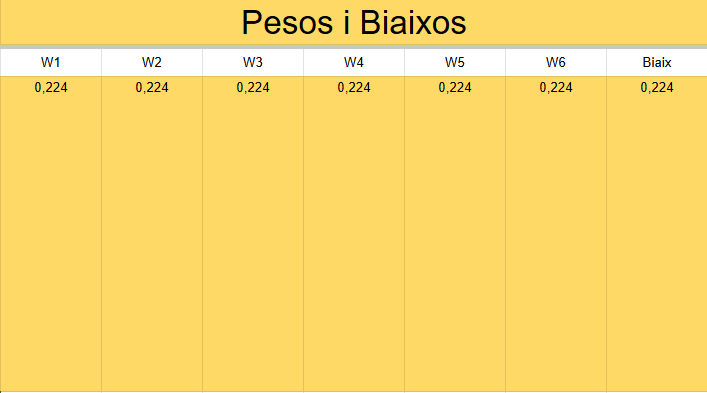
\includegraphics[width=0.7\textwidth]{./figures/Pesos.png}
    \caption{Taula dels pesos}
    \label{f:pesos}
\end{figure}

A la figura~\ref{f:pesos}, observem com queda la taula després d’afegir els pesos als valors d’entrada. Cal afegir sis columnes de pesos, corresponents a les sis entrades, i una columna addicional per al biaix.

\subsection{Funció d'error del model}
Fins ara, tenim les dades d’entrada normalitzades i els pesos inicials assignats. Ara podem aplicar la fórmula utilitzada en les xarxes neuronals per calcular la predicció temporal de la nota final. Cal recordar que la fórmula és la següent:
$$\sum w_i x_i + \text{biaix}$$
Després d’aplicar la fórmula, obtenim la predicció de la nota final, tal com es mostra a la figura~\ref{f:Predicciones}.
% \begin{comment}
\begin{figure}[h!]
    \centering
    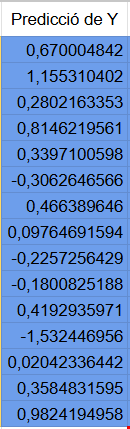
\includegraphics[width=0.18\textwidth]{./figures/Predicciones.png}
    \caption{Prediccions del model}
    \label{f:Predicciones}
 \end{figure}
% \end{comment}
Cal recordar que els valors de la predicció són incorrectes, ja que els pesos assignats són inicialment aleatoris. Per aquest motiu, el següent pas de la pràctica consisteix a entrenar el model per millorar els paràmetres. Per fer-ho, apliquem un procés d’optimització que ajusta aquests paràmetres; en aquest cas, utilitzarem l’algoritme de gradient descendent.\\

Comencem afegint més columnes a la nostra taula del full de càlcul. Si restem els valors de la predicció ($Y$) dels valors reals ($y$), obtenim la diferència entre les notes reals dels alumnes i les prediccions del model.\\

A la figura~\ref{f:errors} es mostren dues columnes addicionals: la columna \textit{error} emmagatzema els errors del model, mentre que l’altra columna conté els mateixos errors en valor absolut, és a dir, tots els valors són positius. D’aquesta manera, resulta més fàcil visualitzar la magnitud dels errors i facilitar els càlculs necessaris per ajustar els paràmetres.\\

Després de crear aquestes taules, calculem la mitjana dels valors de la columna d’errors en valor absolut. El resultat d’aquesta mitjana ens permet avaluar si, en cada iteració, l’error està augmentant o disminuint. Com més baix sigui aquest valor, més precisa serà la predicció.

\begin{figure}[h!]
    \centering
    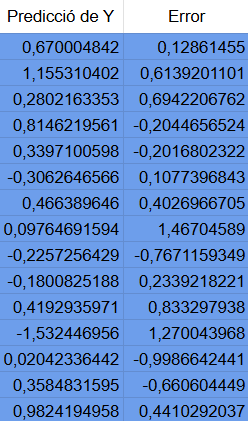
\includegraphics[width=0.28\textwidth]{./figures/Errors.png}
    \caption{Erros de la predicció}
    \label{f:errors}
\end{figure}

\subsection{Canvis dels paràmetres}
Un cop tenim la funció d’error de la primera predicció, el pas següent és entrenar el model per ajustar els valors dels pesos i del biaix, de manera que les prediccions següents siguin més precises.\\

Per aconseguir-ho, cal tenir en compte que quan la diferència entre $Y$ i $y$ és més gran, els pesos estan més allunyats dels seus valors ideals. Per tant, necessitem una forma de calcular correctament els ajustos dels pesos en funció de la diferència entre els valors de la predicció i els valors reals.\\

Segons la fórmula de la xarxa neuronal, si el valor d’entrada ($X$) és petit, el seu pes ($W$) també tindrà un impacte petit, ja que es multipliquen. Així, hem de considerar tant la diferència entre la predicció final ($Y$) i el valor real ($y$), com el valor d’entrada ($X$) respecte al seu pes ($W$).\\

Per això, la fórmula que utilitzarem per calcular els canvis dels paràmetres és:

$$\Delta W = (Y_{\text{original}} - Y_{\text{predicció}}) \times X$$
Aquesta fórmula ens permetrà ajustar els pesos i el biaix per millorar progressivament la precisió de la predicció. Aplicant-la a cada una de les dades, obtindrem set columnes addicionals corresponents als ajustos de cada pes i del biaix.

\begin{figure}[h!]
    \centering
    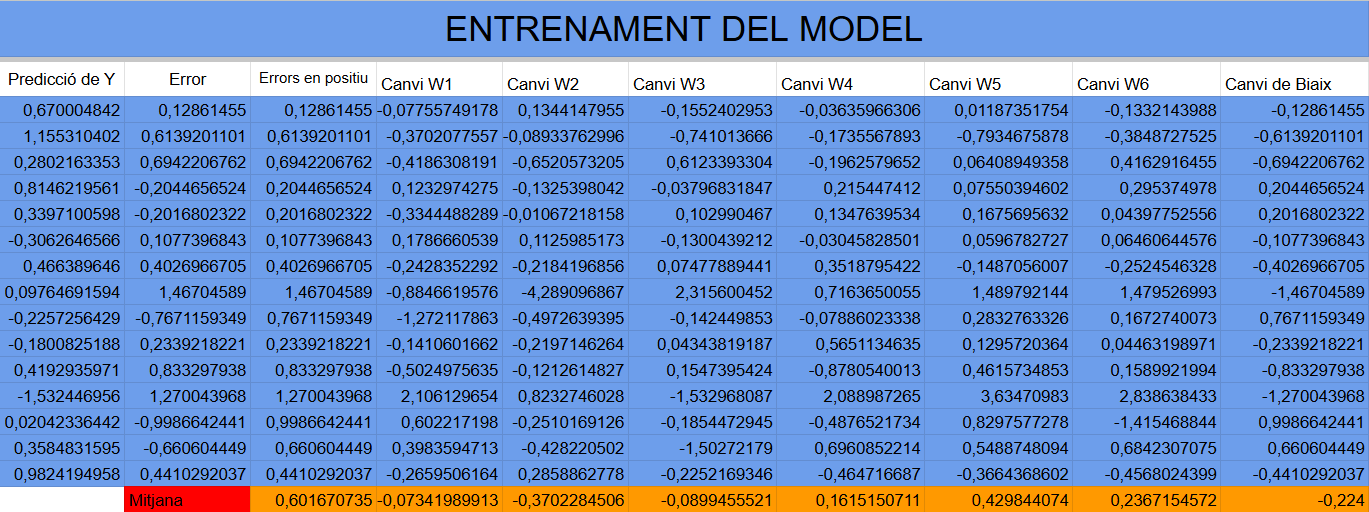
\includegraphics[width=0.9\textwidth]{./figures/Canvis.png}
    \caption{Canvis en els paràmetres}
    \label{f:canvisParametres}
\end{figure}

A la figura~\ref{f:canvisParametres} es mostren aquestes taules. Els canvis del biaix es calculen amb la mateixa fórmula que els dels pesos, però sense multiplicar per cap valor d’entrada, ja que el biaix actua com una entrada constant.

A continuació, calculem la mitjana dels canvis dels pesos. Aquestes mitjanes seran uns dels valors utilitzats per ajustar els paràmetres del model i millorar la precisió de les prediccions.
\vspace{-1.5truecm}
\subsection{La taxa d'aprenentatge}
Abans de començar a entrenar el model, cal parlar d’una variable molt important: la taxa d’aprenentatge. Aquesta taxa és un paràmetre que ajusta la magnitud dels passos que fem per actualitzar els pesos i el biaix del model. El seu valor no pot ser massa gran, ja que podria dificultar trobar el punt de convergència, ni massa petit, ja que alentiria l’entrenament de la xarxa.\\

Normalment, el valor de la taxa d’aprenentatge és 1, però en alguns casos aquest valor pot ser massa gran i augmentar l’error del model. Si això passa, cal reduir progressivament la taxa fins a un punt on l’error de la xarxa disminueixi de manera significativa.\\

Finalment, per calcular els valors finals dels canvis ajustats dels paràmetres, multipliquem la mitjana dels canvis dels pesos per la taxa d’aprenentatg\\
\vspace{-1.8truecm}
\subsection{Èpoques d'entrenament}
Ara passem a entrenar el model. Ho farem utilitzant la mateixa taula que hem creat anteriorment, tal com es mostra en la figura~\ref{f:entrenament}.

\begin{figure}[H]
    \centering
    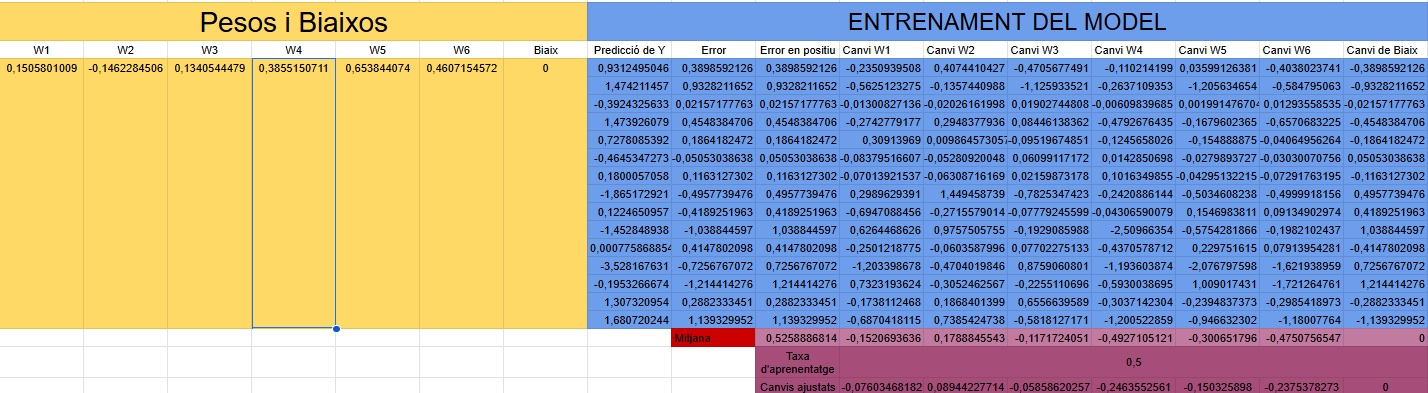
\includegraphics[width=1\textwidth]{./figures/Etapa1.png}
    \caption{Èpoques d'entrenament (Etapa 1)}
    \label{f:entrenament}
\end{figure}

\begin{figure}[H]
    \centering
    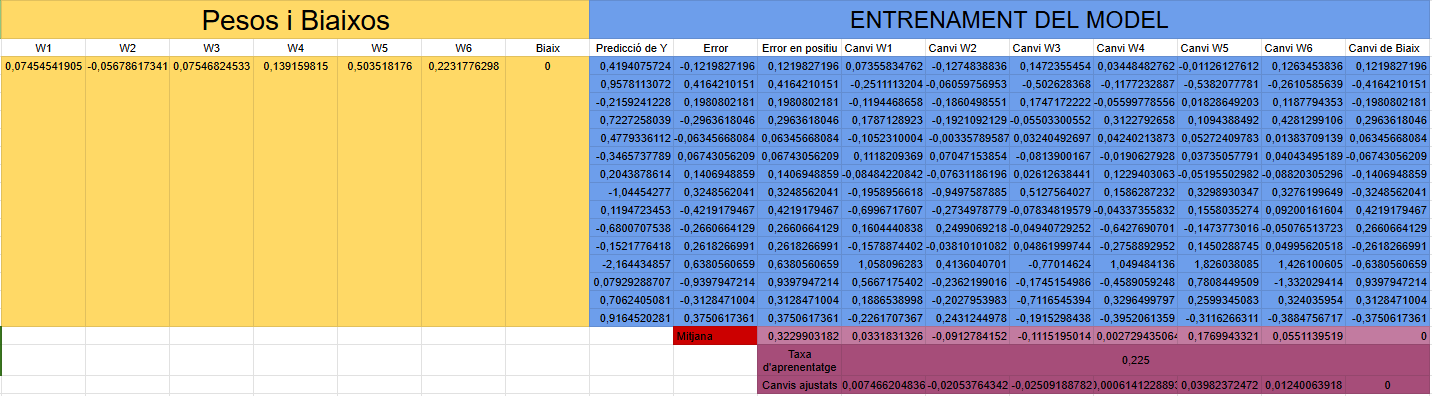
\includegraphics[width=1\textwidth]{./figures/Etapa2.png}
    \caption{Èpoques d'entrenament (Etapa 2)}
\end{figure}

\begin{figure}[H]
    \centering
    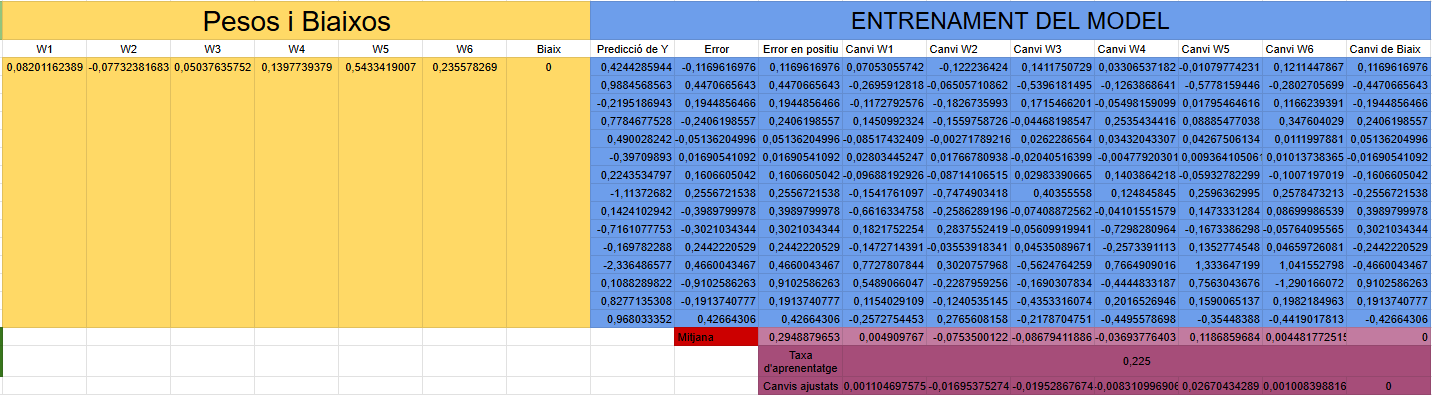
\includegraphics[width=1\textwidth]{./figures/Etapa3.png}
    \caption{Èpoques d'entrenament (Etapa 3)}
\end{figure}

\begin{figure}[H]
    \centering
    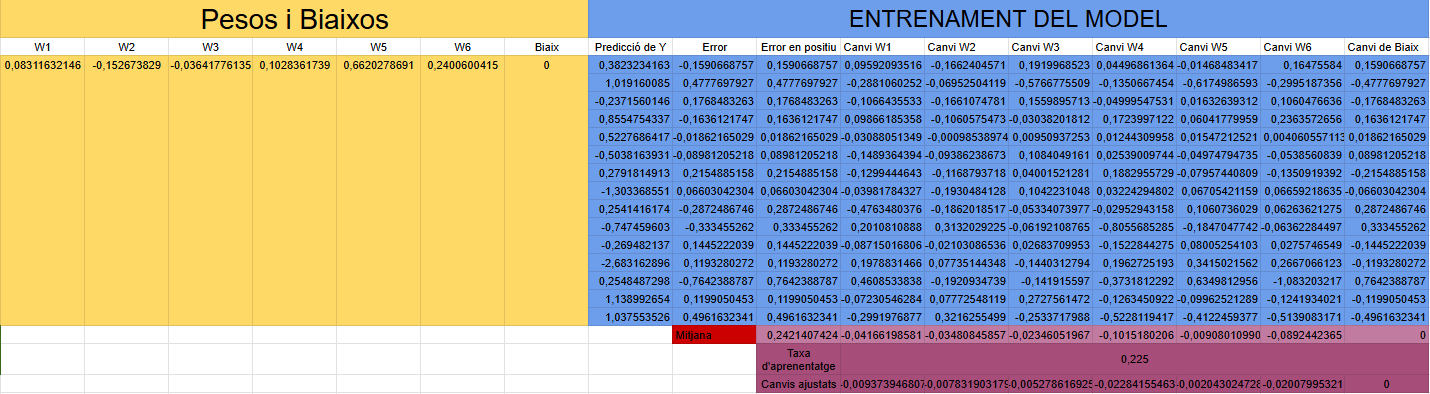
\includegraphics[width=1\textwidth]{./figures/Etapa4.png}
    \caption{Èpoques d'entrenament (Etapa 4)}
\end{figure}

\begin{figure}[H]
    \centering
    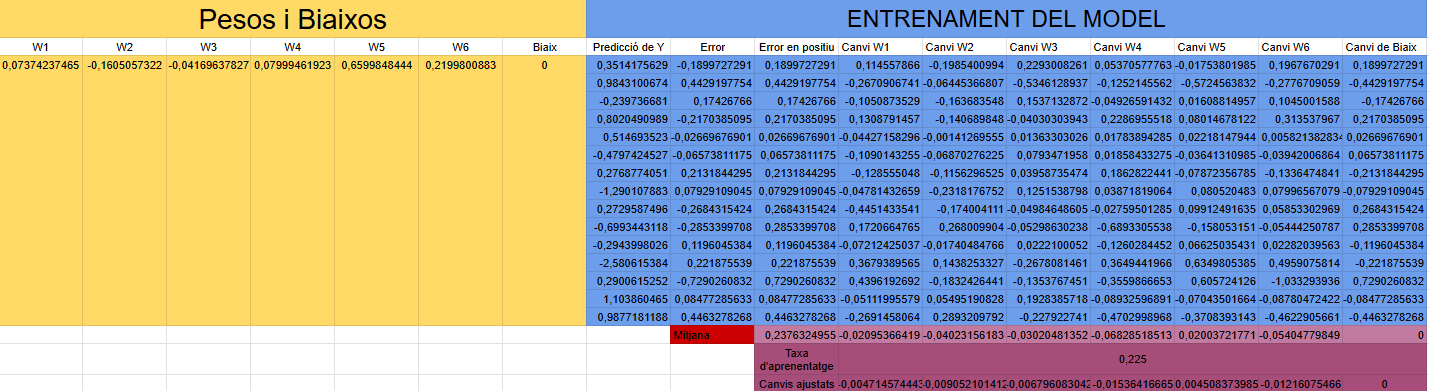
\includegraphics[width=1\textwidth]{./figures/Etapa5.png}
    \caption{Èpoques d'entrenament (Etapa 5)}
\end{figure}

\begin{figure}[H]
    \centering
    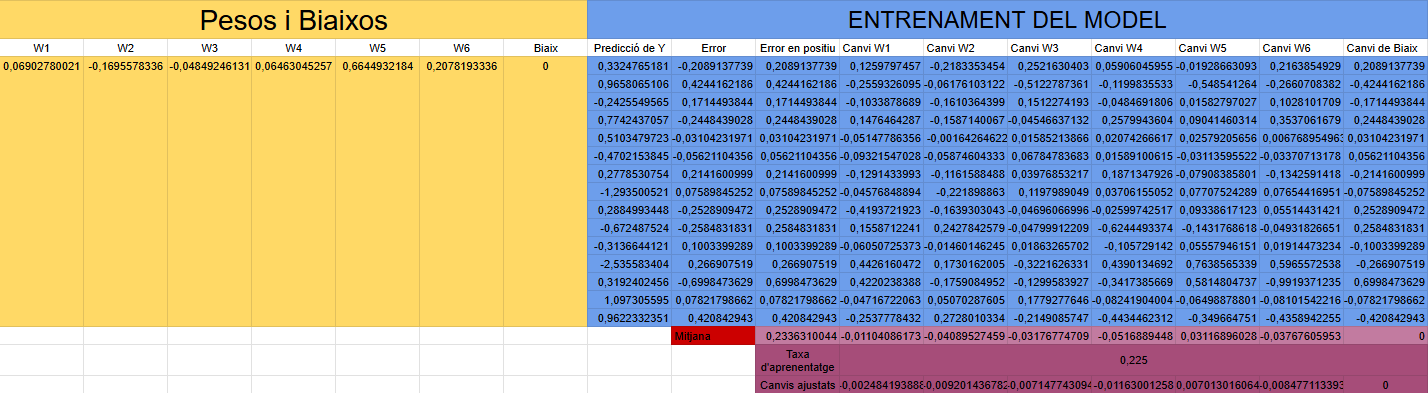
\includegraphics[width=1\textwidth]{./figures/Etapa6.png}
    \caption{Èpoques d'entrenament (Etapa 6)}
\end{figure}

\begin{figure}[H]
    \centering
    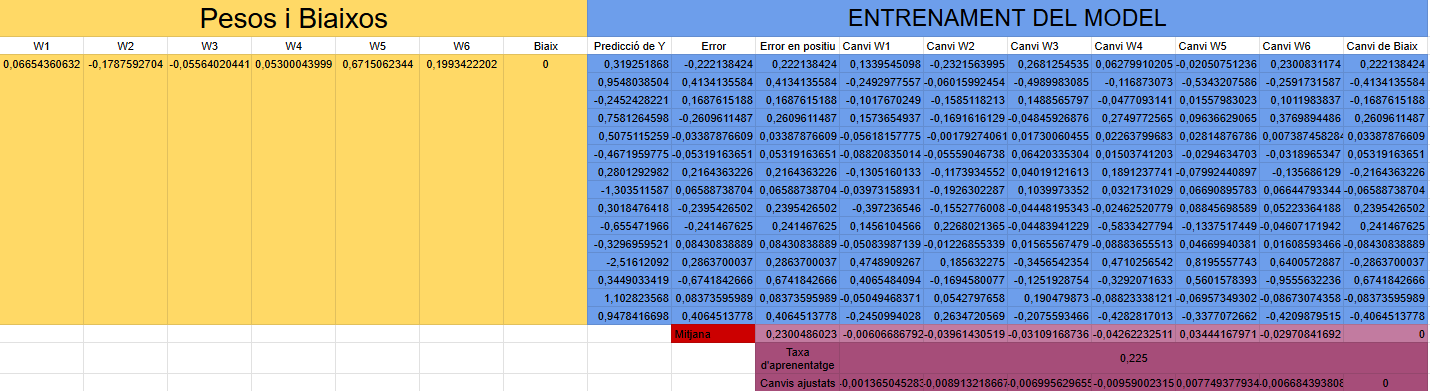
\includegraphics[width=1\textwidth]{./figures/Etapa7.png}
    \caption{Èpoques d'entrenament (Etapa 7)}
\end{figure}

\begin{figure}[H]
    \centering
    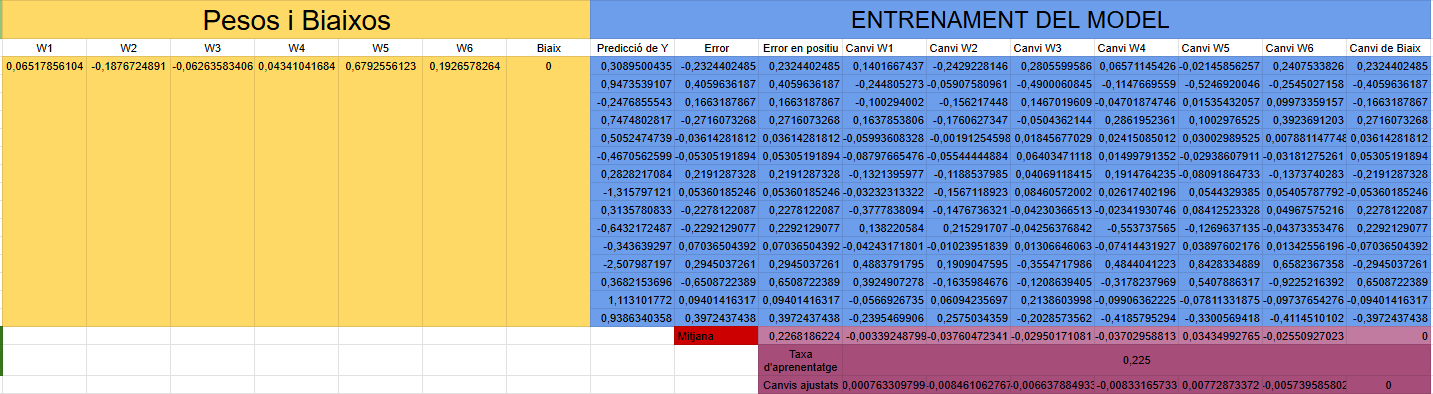
\includegraphics[width=1\textwidth]{./figures/Etapa8.png}
    \caption{Èpoques d'entrenament (Etapa 8)}
\end{figure}

Cada època d’entrenament representa una iteració. Podem observar que els paràmetres de la primera època han canviat respecte als de la taula inicial, que anomenarem època 0, on els paràmetres eren inicialment aleatoris. Per exemple, el valor del primer pes de l’època 1 ($W_1$) es calcula sumant el pes de l’època 0 amb el valor del canvi ajustat.\\

Per avaluar si el model ha millorat, la millor manera és consultar la taula dels errors en valor absolut. Si aquest valor disminueix respecte a l’època anterior, significa que el model està millorant.\\

A partir d’aquí, repetim aquest procés iterativament fins que els canvis en l’error entre èpoques siguin molt petits. Quan això succeeix, podem considerar que el model està pràcticament en el punt de convergència.%, i és important anant ajustant la taxa d'aprenentatge.
\subsection{Resultats a la vuitena iteració}
En aquest cas, han calgut 8 iteracions per arribar al punt de convergència. Hem organitzat els valors de l'error de cada època en una gràfica perquè sigui més fàcil visualitzar els canvis.

\begin{figure}[h!]
    \centering
    \includegraphics[width=1\textwidth]{./figures/Gràfica_error.png}
    \caption{Gràfica dels valors d'error en cada època}
    \label{f:errorsEpoca}
\end{figure}

A la figura~\ref{f:errorsEpoca} es pot apreciar que l’error disminueix de manera significativa entre l’època 0 i l’època 4. A partir de la cinquena època, però, l’error pràcticament no varia. Tot i ajustar la taxa d’aprenentatge diverses vegades, l’error només disminueix molt lentament fins a arribar a l’etapa 8. Això indica que el model ja no pot ajustar més els pesos.

\section{Resultats de la xarxa neuronal amb Python}
\begin{comment}
\fbox{\parbox{0.9\linewidth}{\textbf{\emph{
    Hem de tenir en compte que les notes finals dels alumnes estan arrodonides;
    per tant, considerarem que la predicció ha estat encertada si té un marge
    d'error menor a 0,5.
  }}}%
}
\end{comment}
Un cop finalitzada la construcció de la xarxa neuronal, avaluem el seu rendiment, que assoleix una precisió del 93,75\%. Aquest valor es calcula considerant com a correctes totes les prediccions amb un marge d’error inferior a 0,5 punts, ja que les notes dels alumnes estan arrodonides. Mitjançant l’ús d’un full de càlcul, podem organitzar i analitzar les dades obtingudes de manera estadística.

\begin{figure}[h!]
 \centering
 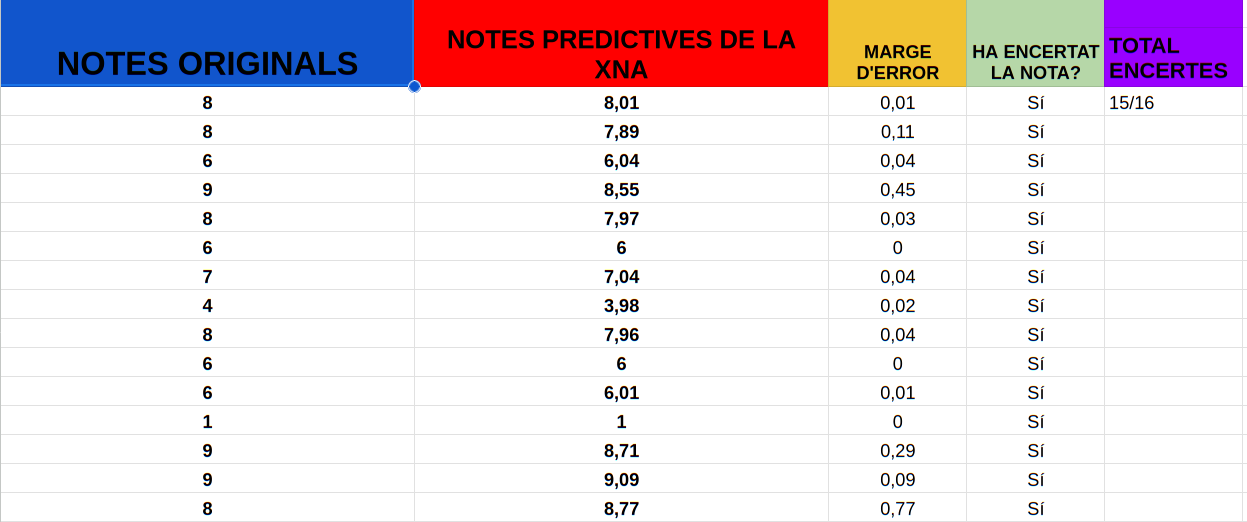
\includegraphics[width=1\textwidth]{./figures/Resultats.png}
 \caption{Resultats obtinguts per la xarxa neuronal amb Python}
 \label{f:resultats}
\end{figure}


\section{Resultats de la xarxa neuronal en full de càlcul}\label{sec: full de càlcul}
Després de completar totes les etapes, els pesos s’han ajustat correctament. Tot i que l’error no ha arribat exactament a zero, és suficientment petit com per considerar-lo acceptable. A la figura següent podem veure els valors finals dels pesos del model.

\vspace*{1truecm}
\begin{figure}[H]
    \centering
    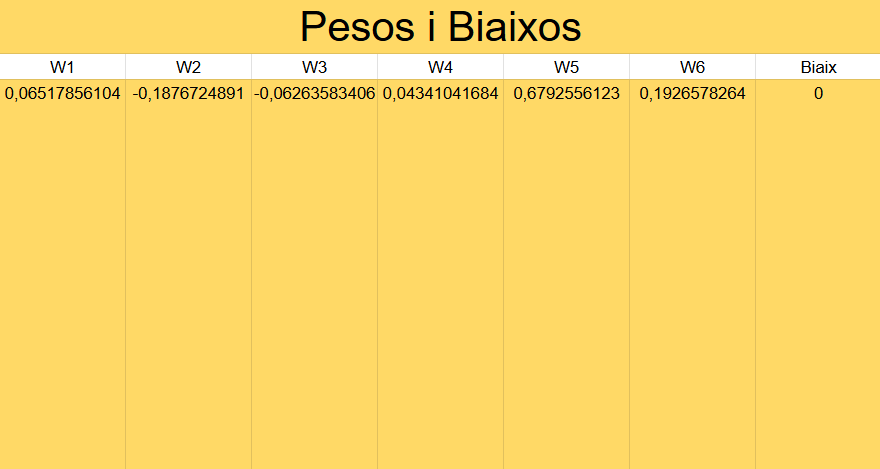
\includegraphics[width=0.9\textwidth]{./figures/Pesos_finals.png}
    \caption{Pesos finals del model}
\end{figure}
Amb aquests pesos, el model hauria de ser capaç d’obtenir prediccions precises de la nota final dels alumnes. Per obtenir els valors finals de la predicció, cal convertir els valors normalitzats de la columna de predicció $Y$ de l’última etapa a valors reals, utilitzant la mateixa fórmula que vam emprar per normalitzar les dades.
$$z = \frac{x - \mu}{\sigma}$$

\vspace*{1truecm}
\begin{figure}[h]
    \centering
    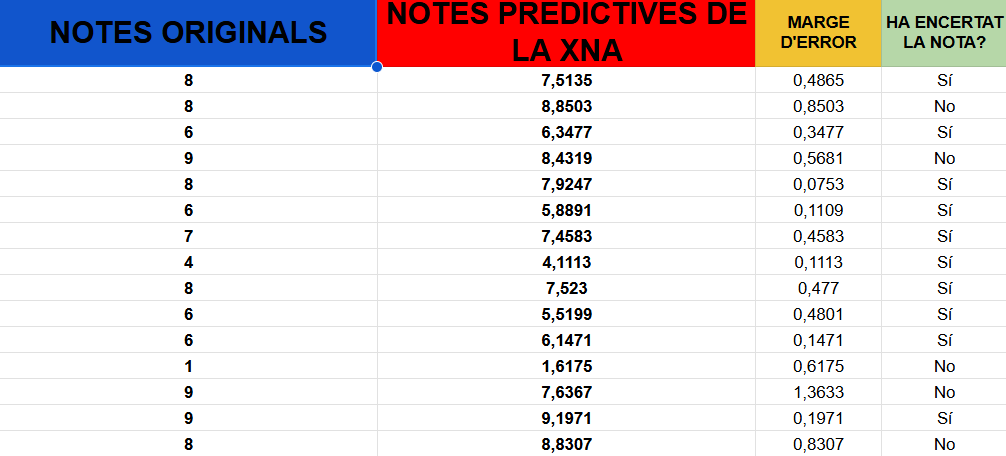
\includegraphics[width=1\textwidth]{./figures/Resultat_final.png}
    \caption{Prediccions finals de la pràctica}
    \label{f:resulat_full}
\end{figure}

\vspace*{1truecm}
A la figura~\ref{f:resulat_full}, després de desnormalitzar els valors, he organitzat les notes originals i les prediccions finals en taules per facilitar la seva visualització. A un costat es mostren les notes reals i a l’altre, les notes predictives.\\

D’aquestes comparacions es mostra que la xarxa neuronal ha encertat 10 notes de 15, cosa que correspon a una precisió aproximada del 66,7\%.

\section{Comparació resultats Python i Full de càlcul}

A continuació, comparem les dues xarxes neuronals per determinar quina és més eficient:

\begin{itemize}

\item \textbf{Precisió:} Un dels factors més rellevants a l’hora de crear una xarxa neuronal predictiva és el seu percentatge d’encert. En aquest cas, la xarxa neuronal implementada amb Python ha assolit una precisió del 93,75\%, molt superior a la del full de càlcul, que ha estat del 66,7\%.

\item \textbf{Coneixements previs:} Crear una xarxa neuronal amb Python requereix coneixements de programació; aprendre el llenguatge és indispensable per implementar la xarxa. En canvi, la xarxa feta amb full de càlcul no necessita coneixements de programació.

\item \textbf{Dificultat:} Segons la nostra experiència, elaborar una xarxa neuronal amb full de càlcul és més senzill que fer-ho amb Python. Amb Python cal codificar tot el procés manualment, mentre que amb el full de càlcul el procés resulta més intuïtiu i mecànic.

\item \textbf{Temps d’elaboració:} El temps necessari per crear una xarxa amb Python depèn de l’habilitat en programació; una persona àgil i experimentada pot completar-la en poc temps. Amb un full de càlcul, malgrat que els càlculs es realitzen automàticament, les etapes s’han de completar manualment, fet que fa que el procés sigui més repetitiu i llarg.

\item \textbf{Visualització:} En una xarxa implementada amb un llenguatge de programació, tot està automatitzat, per la qual cosa no es veu el procés complet fins al resultat final. En canvi, amb el full de càlcul, tot el procés es construeix manualment, mostrant tots els càlculs intermedis i fent-lo molt més didàctic.

\end{itemize}


